\documentclass[
  11pt,
  letterpaper,
   addpoints,
   %answers
  ]{exam}

\usepackage{../exercise-preamble}

\begin{document}

\noindent
\begin{minipage}{0.47\textwidth}

\includegraphics[width=\textwidth]{../fcfm_die}
\end{minipage}
\begin{minipage}{0.53\textwidth}
\begin{center} 
\large\textbf{Electromagnetismo Aplicado} (EL3103-1) \\
\large\textbf{Control 1} \\
\normalsize Prof.~Benjamin Jacard H.\\
\normalsize Prof.~Aux.~Erik Saez A.
\end{center}
\end{minipage}

\vspace{0.5cm}
\noindent
\vspace{.85cm}

\begin{questions}
    %%%%%%%%%%%%%%%%%%%%%%%%%%%%
    \question     
    En un cilindro de radio \( a \) y permeabilidad \( \mu \), se tiene un enrollado superficial de \( N \) vueltas y corriente \( I \). Las vueltas están distribuidas adecuadamente de modo de sintetizar aproximadamente una densidad de corriente superficial:
    \begin{equation}
    \vec{J}_s = J_{s0} \sin\theta\, \vec{K}.
    \end{equation}
    Se cumple que:
    \begin{equation}
    NI = \int_{\theta=0}^{\pi} J_s(\theta)\, a\, d\theta.
    \end{equation}
    
    \begin{enumerate}
        \item[i)] El potencial magnético escalar \( \phi_m \) y el campo \( \vec{H} \) en los medios \( 1 \) y \( 2 \).
        \item[ii)] La inductancia del enrollado en base a la energía acumulada en el campo magnético, por unidad de longitud del cilindro.
    \end{enumerate}
    
    \noindent\textbf{Nota}: La solución de la ecuación de Laplace \( \nabla^2 \phi_m = 0 \) adecuada para este problema es de la forma:
    \begin{align}
    \phi_m(r,\theta,z) = \phi_m(r,\theta) = \left( A r + \frac{B}{r} \right) \cos\theta.
    \end{align}
    
\begin{center}
    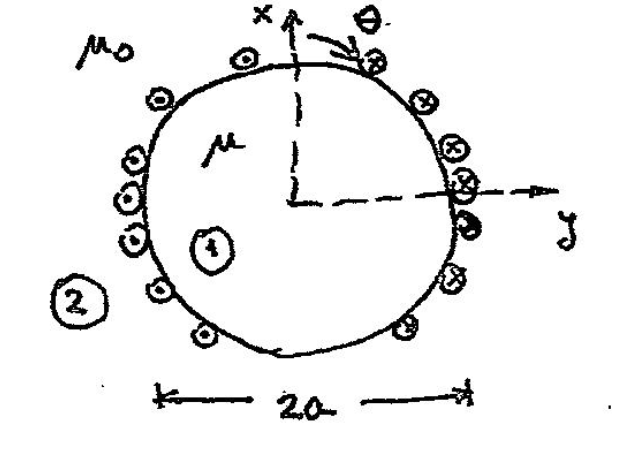
\includegraphics[width=0.35\textwidth]{Control_1_2}
    \captionof{figure}{Esquema del problema}
\end{center}
    %%%%%%%%%%%%%%%%%%%%%%%%%%%%
    \begin{solution}
   
    \end{solution}
    %%%%%%%%%%%%%%%%%%%%%%%%%%%
    \newpage
    \question  
   
    Para el condensador de placas en ángulo de la figura, con dieléctricos perfectos de permitividades \( \varepsilon_1 \) y \( \varepsilon_2 \), determinar:

    \begin{enumerate}
        \item[i)] Potencial \( \phi(r,\theta,z) \) y campo \( \vec{E}(r,\theta,z) \) en los medios \( 1 \) y \( 2 \).

        \item[ii)] Densidad de carga superficial \( \rho_s \) y carga total \( Q \) en las placas conductoras.
    
        \item[iii)] Capacidad del condensador en base a la energía acumulada en el campo eléctrico.
     
    \end{enumerate}
    
    \noindent\textbf{Nota}: Despreciar efectos de borde (campos fuera de los dieléctricos).
    
    La solución adecuada de \( \nabla^2 \phi = 0 \) es de la forma:
    \begin{align}
    \phi(r,\theta,z) = \phi(\theta)= A\theta + B.
    \end{align}
    \begin{center}
        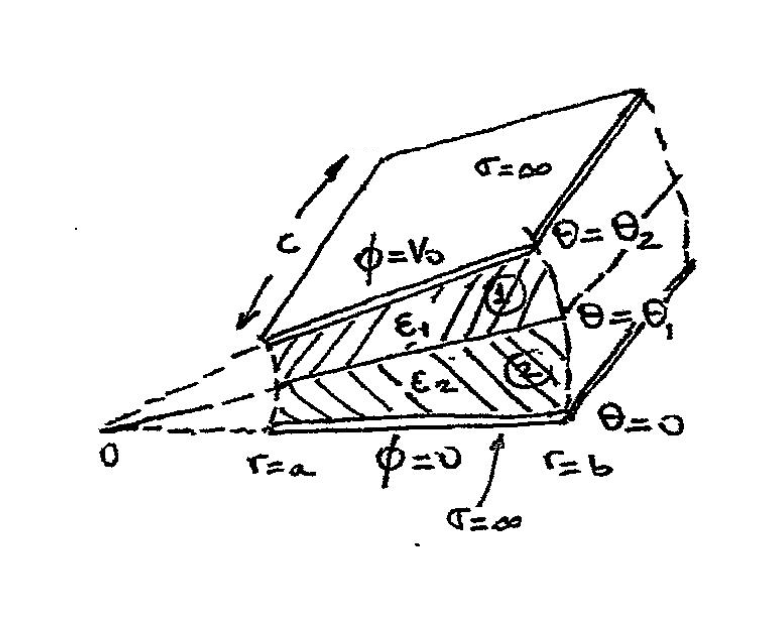
\includegraphics[width=0.45\textwidth]{Control_1_1}
        \captionof{figure}{Esquema del problema}
    \end{center}
    %%%%%%%%%%%%%%%%%%%%%%%%%%%
    \begin{solution}
       a
\end{solution}
%%%%%%%%%%%%%%%%%%%%%%%%%%%

\end{questions}
%%%%%%%%%%%%%%%%%%%%%%%%%%%

\end{document}